%!TEX root = ../thesis.tex
%*******************************************************************************
%*********************************** Sixth Chapter *****************************
%*******************************************************************************

\chapter{Investigation of changes of the basal impedance signal}  %Title of the First Chapter
\label{chapter basal}

\ifpdf
\graphicspath{{Chapter6/Figs/Raster/}{Chapter6/Figs/PDF/}{Chapter6/Figs/}}
\else
\graphicspath{{Chapter6/Figs/Vector/}{Chapter6/Figs/}}
\fi

\rvmynote{This is the introduction of the basal impedance measurements. I have to change the introduction to flow more accordingly.}
One of the characteristics of the impedance plethysmography device is the ability to measure the basal impedance of any tissue with a cylindrical shape, in this case, the left forearm. The data collected using the procedure described in chapter \ref{chapter procedure} provided characteristics of the impedance from eight participants. During the whole test, four regions contained information about the baseline impedance either previous or after an upper arm occlusion, which are the regions 1, 3, 5 and 7 of the data sets. 

The results presented in this chapter describe the different elements that may affect the resistive baseline impedance during a measurement. For this, the baseline measurements were extracted from the whole data from the regions previously explained. It must be noticed that the baseline regions consists on \SI{5}{\minute} of recordings either before or after an occlusion. Hence, \SI{2}{\minute} of recovery to baseline were allowed before extracting the data to be analysed. Therefore, during the post-processing, the last three minutes of the baseline signals were gathered and analysed per participant. The information collected shows insights of what noises may affect the measurements and what frequency components alter the baseline signal. 

\rvmynote{This is the introduction of the changes of basal impedance measurements. I have to change the introduction to flow more accordingly. Flowing with the other section.}

Venous occlusion plethysmography requires occluding the proximal section of the arm, obstructing the return of the venous blood. This kind of examination is used to assess peripheral vascular diseases such as deep venous thrombosis.  In this study, the upper arm was occluded using a cuff at three different levels to recreate the effect of venous occlusion plethysmography.

As explained in chapter \ref{chapter procedure}, the experiment proceeds by recording five minutes of baseline signal followed by a level of occlusion. From there, regions 1, 3, 5 and 7 refer to the five minutes of baseline waveform. On the other hand, regions 2, 4 and 6 are equivalent to venous, partial arterial and total occlusions. In average the level of occlusion for each area were \SI{55}{\mmHg}, \SI{94.62}{\mmHg}, and  \SI{136.25}{\mmHg} respectively. Table  \ref{tbl: venous occlusions} describes the levels of occlusion for each participant. 

During the occlusion of the venous return in the upper arm, the blood pools within the veins in the forearm increasing its volume. This increase of volume reflects a change of resistivity as a more conductive medium is present. 

When the occlusion pressure is below diastolic occlusion, it is only affecting the blood return towards the hearth, but the arterial blood is still coming in the arm. In contrast, blocking the upper arm between diastolic and systolic pressures not only prevents the venous blood return but also constricts the income of arterial pressure into the arm. In the case of total occlusion when the cuff's pressure is above systolic pressure, both venous and arterial flows are blocked. 

This section described in detail the change of impedance in each region. Also, from the data obtained the estimation of blood flow is estimated.


%%********************************** % Section 6.1 ******************************************
\section{Basal impedance results}
\label{section basal 1}
As it can be seen from the instrument's block diagram (see figure \ref{fig:block}), the iPG device provides an output signal denominated $Z_{DC}$ which is equivalent to the mean impedance value of the elbow to wrist segment. The iPG device was able to detect the forearm's segment impedance quite remarkably. The values obtained fell within the resistive value in the tens Ohms as estimated by the literature \cite{dai2009vivo, faes1999electric, grimnes1983impedance}. This section will describe the elements that affected the baseline impedance of the signal. For this, the data was portioned to the last \SI{3}{\minute} of the recorded baselines. By doing this, the effect of the movement and recovery time of the forearm after releasing the occlusion was diminished. 

It must be remarked that the baseline signal also contains an AC component equivalent to the arterial pulses. For the analysis of this section, the APA information was suppressed. Only, the resistivity mean value also known as basal impedance was computed, which is equivalent to the value of $R_B$ as in Nyboer's equation \ref{eq:nyober dV} or the foot of the signal in the plethysmography waveform. In other words, it is the value of the impedance before circulation occurs and is composed of the impedance contribution of bone, muscle, fat, skin and residual blood within the vessels \cite{dai2009vivo}. 

Figure \ref{fig:Basal statistics} shows the statistic values of the median basal impedance during the regions 1, 3, 5 and 7. The mean resistive baseline impedance of all the participants was \SI{78.62(1461)}{\ohm}. The impedance was entirely independent of the person sex.  

\begin{figure}[!htbp]
	\centering
	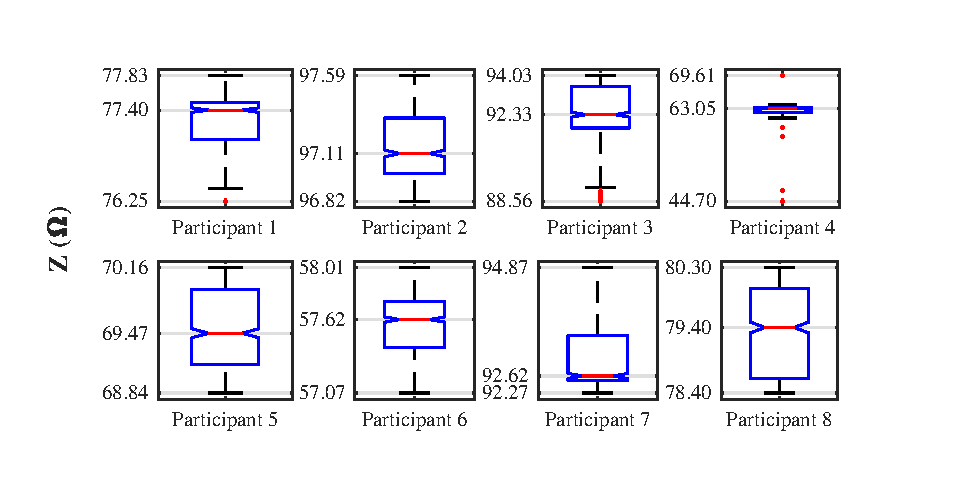
\includegraphics[width=0.85\textwidth,keepaspectratio]{figure_b_1}    
	\caption[Mean basal impedance boxplot]{Mean basal impedance of all the participants during the last \SI{3}{\minute} of the baseline regions 1, 3, 5 and 7.}
	\label{fig:Basal statistics} 
\end{figure}

Artefact motion caused the outliers of the readings. As it can be noticed from the plot, participants 1, 3 and especially 4 presented deviated points during the study. Also, participants 3, 4 and 8 showed the largest distribution between interquartile values larger than \SI{1}{\ohm} (mean \SI{1.41(39)}{\ohm}). The rest of the participants showed a distribution within first and third interquartile of about \SI{0.57(27)}{\ohm}. 

%%********************************** % Section 6.2 ******************************************
\subsection{Relation between geometry and mean basal impedance}
\label{senction basal 2}
There are different aspects of the geometry that could affect the impedance reading. There have been several studies which demonstrated how the distance between electrodes affects readings on tissue \cite{kun2000effects, yamamoto1992impedance}. This study portrayed that he forearm's circumference and the distance between the potential electrodes influences the impedance measurement. Figure \ref{fig:C_vs_Z} indicates that there is an inverse relation between circumference and impedance (slope \SI{-0.072}{\centi\meter\per\ohm}). The smaller the forearm's circumference, the higher the resistivity. On the other hand, there is a direct relation between the distance between the potential electrodes and the resistivity of the segment (slope \SI{0.055}{\centi\meter\per\ohm}) as depicted in \ref{fig:l_vs_Z}.

Moreover, when comparing total volume measured to the mean resistivity of the segment (see figure \ref{fig:Ve_vs_Z}), the impedance tends to increase when the forearm's segment volume decreases (slope \SI{-0.622}{\cubic\centi\metre\per\ohm}). Which is in agreement with the fact that when more tissue is involved in the measurement, the more conductive path for the current, reducing the total impedance. However, this can not be seen as an entirely linear relationship as the impedance value can be affected by the amount of adipose tissue. Having two different arms with same dimensions, the one with more fat will produce a different basal impedance reading that the one with a higher muscular tone. 

\begin{figure*}[!b]
	\centering
	\begin{subfigure}[t]{0.48\textwidth}
		\centering
		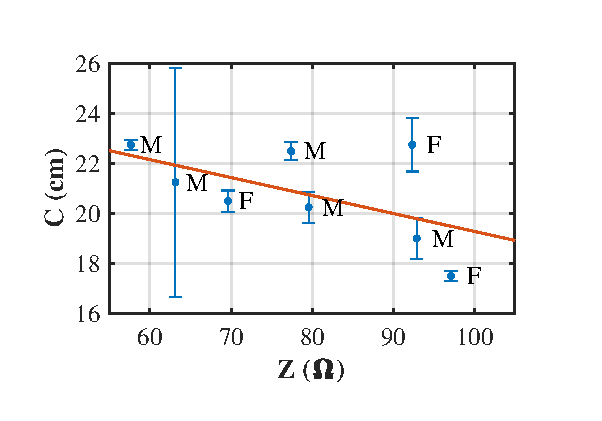
\includegraphics[width=7cm]{figure_b_2a}
		\caption{Relationship between forearm circumference and mean basal impedance}
		\label{fig:C_vs_Z}
	\end{subfigure}%
	~ 
	\begin{subfigure}[t]{0.48\textwidth}
		\centering
		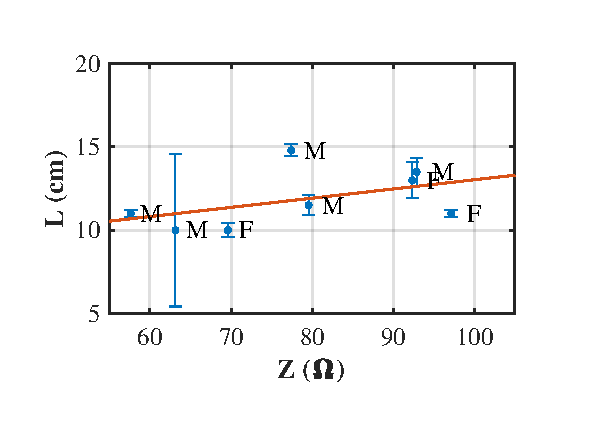
\includegraphics[width=7cm]{figure_b_2b}
		\caption{Relationship between distance sensing electrodes and mean basal impedance}
		\label{fig:l_vs_Z}
	\end{subfigure}
	~ 
	\begin{subfigure}[t]{0.48\textwidth}
		\centering
		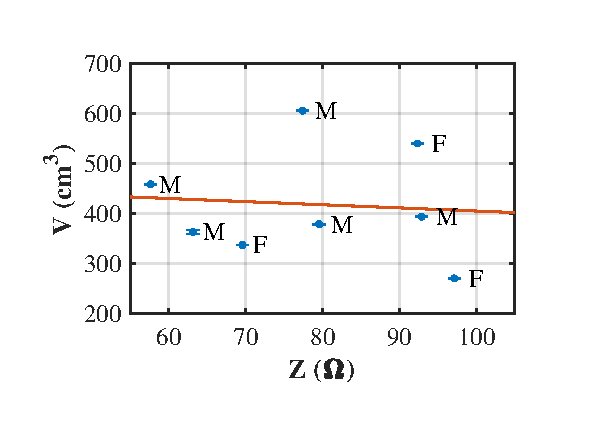
\includegraphics[width=7cm]{figure_b_2c}
		\caption{Relation between forearms segment volume and mean basal resistivity}
		\label{fig:Ve_vs_Z}
	\end{subfigure}
	\caption{Relation between circumference, length and total segment's volume and mean basal impedance}
	\label{fig:relation_geometry_vs_impedance}
\end{figure*}

%%********************************** % Section 6.3 ******************************************
\section{Basal impedance changes between measurements}
\label{senction basal 3}
There are different artefacts that can alter the basal impedance during a measurement such as either motion or respiration movement \cite{pandey2006cancellation, swanson1983errors, ansari2010impedance, rosell1995reduction}. In this section will analysed how much the basal impedance changes between measurements. All the participants were asked to stay still for the whole duration of the test. However, in practice, this is not completely possible as keeping the same position for a prolonged period of time can be quite tiring. Inflating the cuff to a pressure above diastolic level may cause discomfort to the participants like tingling sensation or even pain, a normal response of the body is to move the limb to restore the blood flow. The first \SI{2}{\minute} of the baseline impedance readings may be affected by the rearrange of the participant's position especially after the occlusion of the upper arm. Moreover, the blood flow restriction also induced a physiological response which needed some time to go back to baseline value. Hence, the baseline data after \SI{2}{\minute} is used for this analysis, allowing enough time to recover. 

The data used for the analysis was compiled by extracting the lower envelope of the raw basal impedance. The command envelope in Matlab \cite{MATLAB:2016} allows to isolate the desired signal. Figure \ref{fig:Basal Regions} shows the waveform extracted with the respective mean value for each region per participant. The region 1 applies to the time where the initial reference was recorded, in total \SI{5}{\minute} were recorded but the last \SI{3}{\minute} of data were extracted right before the occlusion between \SIrange{120}{300}{\second}. This basal impedance is the reference to the other readings as was not affected by occlusion of any kind. The other sections of the data correspond to the region 3 which is the recovery after venous occlusion, the information extracted belongs to the time slot between \SIrange{ 600}{780}{\second}.  Similarly, the region 5 after partial arterial occlusion retrieving the last \SI{3}{\minute} of data between \SIrange{1080}{1260}{\second}. Finally, the data after total occlusion in region 7 between \SIrange{1560}{1740}{\second}.

Initially, the first thing that can be observed from the figure is the presence of oscillations in the baseline signal. This signal was present in all the participants with subtle frequency variations between each region. The frequency was calculated by extracting the period of the signal as the difference between its peaks. In average the frequency of the oscillation was \SI{0.0685(00027)}{\hertz}. At this point, it is not possible to establish if this is either a common noise coming from the instrument or a physiological response. In the literature, there is not much information about impedance plethysmographic oscillations at this frequency band.  However, a study using laser Doppler flowmetry found that physiological measurements into this frequency spectrum may be related to the sympathetic activity (\SIrange{0.02}{0.06}{\hertz}) \cite{kvandal2006low}. Further investigation has to be performed to discover the roof of this signal. 

Secondly, it is evident that the motion artefact altered some of the measurements. Participants 3 and 4 clearly displayed deviation from their mean values in region 2 and region 4 respectively. In fact, the figure had to be clipped to fit the waveform information properly. On the other hand, it is hard to detect great changes on partaker 1, but region 3 displayed significant variations compared to the other areas. Hence, this qualitative analysis also confirms the quantitative results shown in figure \ref{fig:Basal statistics}.  

\begin{figure}[!htbp]  %fig:rb:all_participants
	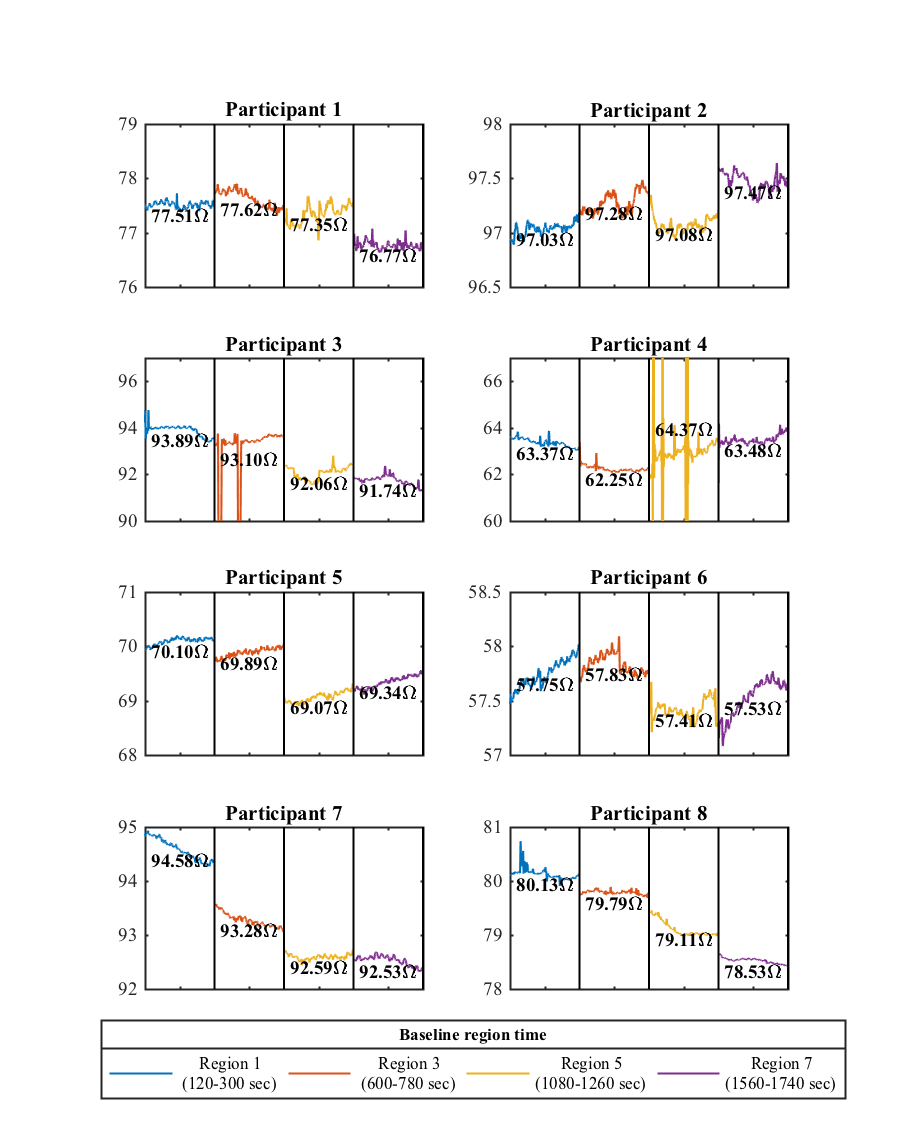
\includegraphics[width=\textwidth,keepaspectratio]{figure_b_3}    
	\caption[Measurements of the basal impedance during the whole study]{Basal impedance of all the participants during the whole study. The data collected has been divided into regions. The regions (1,3,5 and 7) in white colour represent baseline measurements. The shaded areas (regions 2,4 and 6) represent occlusive events.  }
	\label{fig:Basal Regions} 
\end{figure}

Lastly, it is evident that there are variations on the baseline impedance between regions. Also, there is not a clear trend on either the increase or decrease of the basal impedance, except on participants 7 and 8 where there is a decrease on impedance. Big gaps (< \SI{0.8}{\ohm}) between regions can be noticed on participant 5 and participant 7. It is important to determine if the change of impedance is larger than when performing VOP. Therefore, the following section analyses in depth the change of basal impedance and quantifies the changes. 

 
%%********************************** % Section 6.3.1 ******************************************
\section{Basal impedance change between regions}
\label{senction basal 3.1} 
The basal impedance signal contains noises that may deviate the signal from the baseline. As the previous section analysed, the baseline changed between baseline regions. This section will quantify the error compared to the basal impedance at the beginning of the experiment. 

Different factors could affect a bioimpedance reading. One of this is the change of impedance on the electrode-skin interface.  As described in section \ref{section impedance electrodes}, when either the geometry or the area of contact of the electrode changes, it is converted into variations in the total impedance. Also, air pockets that may form between the two elements could contribute to substantial changes in impedance.  Another contributing factor is motion artefact. In this case, the movement of the skin and muscles create different current paths. Hence, the basal impedance deviates from the baseline. 

In an in-vivo setting, it is tough to keep a participant completely motionless for the whole duration of the experiment.  During each baseline, the occlusion of the upper arm caused the participants to move and re-accommodate. Eventually, there was a change of impedance that will be analysed as follows caused by that movement and maybe a physiological response. 

The figure \ref{fig:delta percent} shows the deviation in percentage from the baseline in region 1.  Therefore, the median impedance in this region was the starting point. The data was calculated by extracting the envelope of the impedance waveform. In the figure, each point represents the median value of the resistance and the whiskers the range of the data. The oscillatory component described in the previous section caused the major variations the resistance. It can be appreciated that the baseline impedance tended to decrease in most of the participants except number 2. 

The effect of the motion artefact can be noticed on the large whiskers of some of the participants. For instance, participants 3 and 4 showed the larger ones in region 3 and 5 respectively. Indeed, the data from participant 4 was clipped as the whiskers showed a huge variation of up to \SI{200}{\percent}. It is also important to note that only a few signals were able to return to baseline. For instance, the waveforms that experienced a variation below \SI{0.25}{\percent} were the regions 3 and 4 of participant 1, participant 2 in region 5, participant 4 in region 7 and participant 6 in regions 3 and 7. The rest experience changes between \SIrange{-2.353}{0.441}{\percent} from the baseline region 1. 


\begin{figure}[!t]  %fig:rb:all_participants
	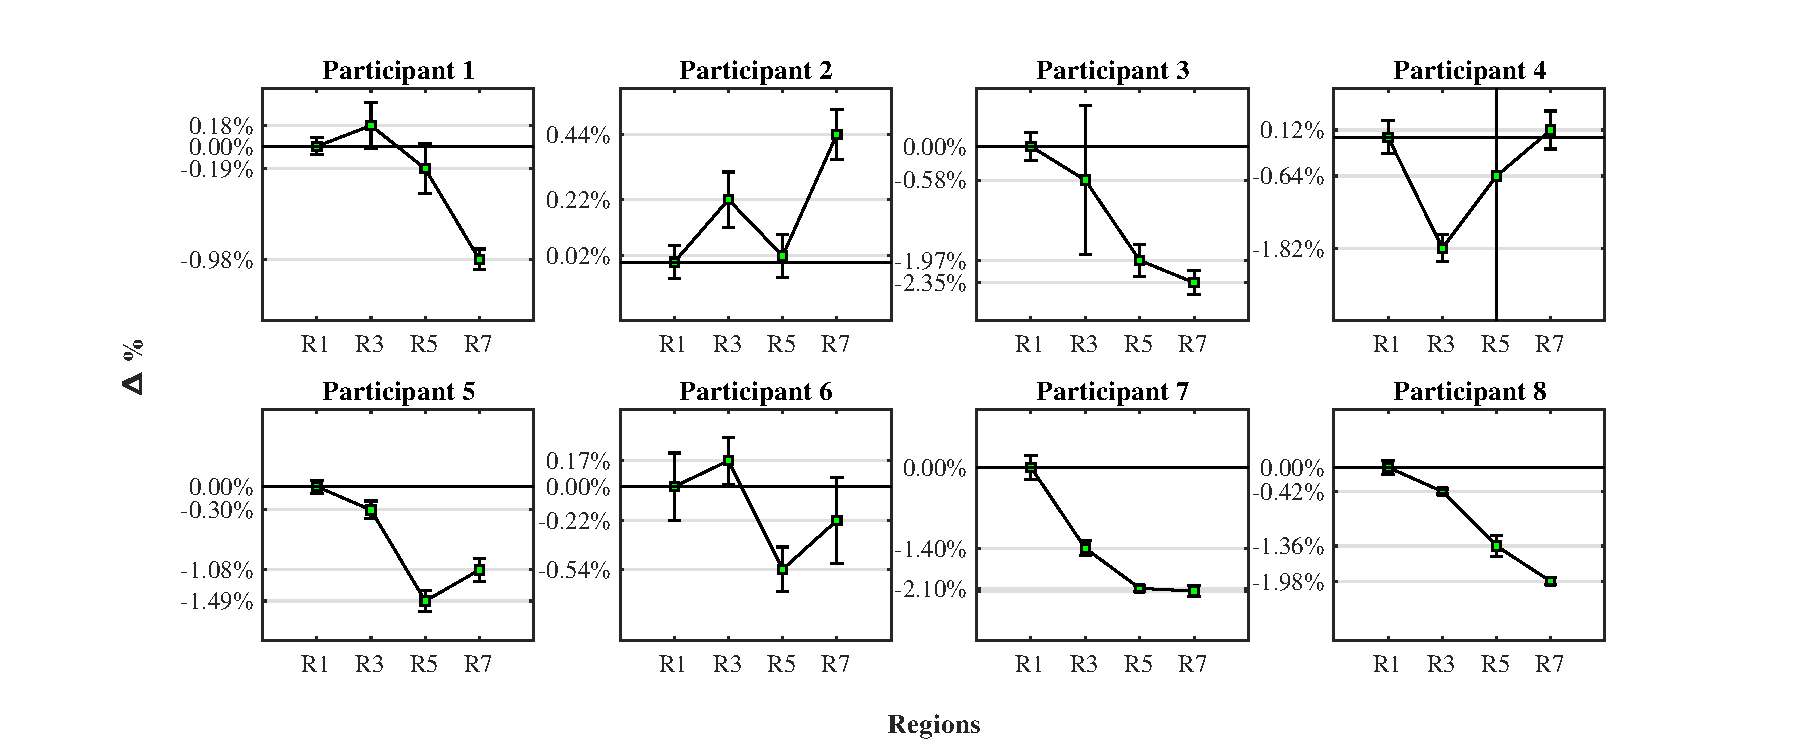
\includegraphics[width=\textwidth,keepaspectratio, trim={2cm 0cm 3cm 0cm},clip]{figure_b_4}    
	\caption[Percentil change of baseline imepdance]{Deviation of the basal impedance for all the participants compared to region 1. Each plot shows how much the impedance increase or decrease against the reference value for regions 3, 5 and 7. }
	\label{fig:delta percent} 
\end{figure}

The table \ref{tbl:change imepdance} shows the range and mean of changes of impedance for all the participants. The average impedance of the whole study was \SI{-0.6384}{\percent} with a range of about \SI{1.5264}{\percent}. Certainly, participants 1, 2 and 7 showed the least impedance change with less than \SI{0.25}{\percent}, whereas the second increased and the others decreased.  A change between \SIrange{0.25}{1}{\percent} was experienced by participants 4, 5 and 8. Finally participants 3 and 7 showed the largest change of impedance of more than \SI{1}{\percent}. 

\begin{table}[!htbp]
	\caption[Range and mean change of impedance of each participant]{Mean and range of the impedance change for each participant.}
	\label{tbl:change imepdance}
	\centering \small
	\begin{tabular}{lcc}
		\toprule
		&\textbf{range ($\Delta \%$)}
		&\textbf{mean ($\Delta \%$)} \\ \midrule
		Participant 1    &     \SI{1.157}{\percent}    &     \SI{-0.247}{\percent}    \\  
		Participant 2    &     \SI{0.441}{\percent}    &     \SI{0.170}{\percent}    \\  
		Participant 3    &     \SI{2.353}{\percent}    &     \SI{-1.226}{\percent}    \\  
		Participant 4    &     \SI{1.939}{\percent}    &     \SI{-0.584}{\percent}    \\  
		Participant 5    &     \SI{1.489}{\percent}    &     \SI{-0.719}{\percent}    \\  
		Participant 6    &     \SI{0.707}{\percent}    &     \SI{-0.148}{\percent}    \\  
		Participant 7    &     \SI{2.147}{\percent}    &     \SI{-1.412}{\percent}    \\  
		Participant 8    &     \SI{1.979}{\percent}    &     \SI{-0.940}{\percent}    \\ 
		\bottomrule 
	\end{tabular}
\end{table}

%%********************************** % Section 6.4 ******************************************
\section{Statistical analysis of basal impedance}
\label{senction basal 4} 
Identifying when the basal impedance is outside normal levels requires performing a statistical analysis. By using all the percentage deviation ($\Delta \%$) from the initial baselines as the data range, it was calculated normal probability density function (PDF). Using the Matlab command \textit{normfit} was computed the normal distribution from the $\Delta \%$. The calculation returned a $\mu = -0.6384$ and a $\sigma = 0.8518$. By plotting the probability distribution function can be seen how the probability distributed. Then by using the $\sigma$ obtained from the data, a new PDF was calculated centred at $\mu = 0$. As result, the PDF produces a similar data distribution where the confidence band (\SI{95}{\percent}) were calculated at $\pm 1.96 \times\sigma$.

Figure \ref{fig:basal pdf} shows the PDF obtained from the data and the new one calculated. The yellow plot shows the confidence area from the baseline. Therefore, the confidence band is between $\Delta \% = \pm 1.66 \%$. In other words, all the changes of impedance within this confidence band can be considered as statistically within normal limits. 

By comparing the results showed from the PDF calculated, most of the participants were within that range. Nevertheless, some partaker's regions are out from this confidence band. For example, regions 5 and 7 in participants 3 and 7, region 3 of participant 4 and region 7 of participant 8.

\begin{figure}[!htbp]  %fig:rb:all_participants
	\centering
	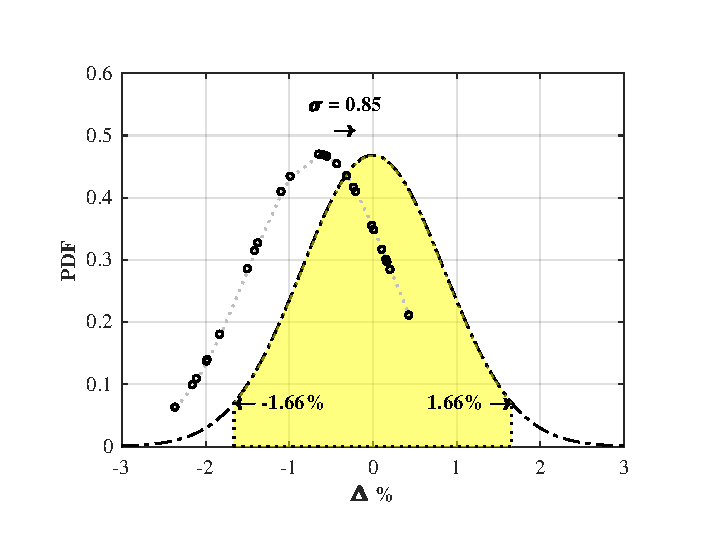
\includegraphics[width=12cm,keepaspectratio, trim={0cm 0cm 0cm 0cm},clip]{figure_b_5}    
	\caption[Percentil change of baseline imepdance]{Deviation of the basal impedance for all the participants compared to region 1. Each plot shows how much the impedance increase or decrease against the reference value for regions 3, 5 and 7. }
	\label{fig:basal pdf} 
\end{figure}


\section{Change of basal impedance during occlusion}
\label{section occlusion 1}
From the data obtained in the experimental procedure, different data regions were extracted according to the kind of occlusion applied. The data were separated in this section into the readings from venous occlusion, partial arterial occlusion (PAO) and total blockage. 

The analysis of the data has to be performed only on the basal impedance. Similarly, as the previous chapter, the arterial pulses were eliminated from the signal. Only, the lower envelope of the impedance signal was used to perform this investigation. 

The data set for this study was subdivided as follows: two minutes of data before the occlusion as the baseline reference, then three minutes of occlusion followed by two minutes of data after releasing the cuff's pressure. 

\subsection{Changes of impedance during venous occlusion}
\label{section occlusion 1.1}
As expected, the basal impedance dropped while performing venous occlusion in each participant. As figure \ref{fig:venous statistics impedance} confirms, all the partakers experienced a decrease in their basal impedance during the region 2 of the experiment. The boxplot shows the three regions that took part of this part of the study. The data of the region 1 (\textit{R1}) were the last \SI{2}{\minute} of the initial baseline (\SIrange{180}{300}{\second}). Thereafter, it is the venous occlusion in region 2 (\textit{R2}) during \SI{3}{\minute} at the pressure levels describe by the column \textit{occlusion 1} in \ref{tbl: venous occlusions}, it is clear that the median resistance value decreased. Analysing this candle-stick can be described that the larger the distribution of the upper and lower quartile, the greater the resistance drop as registered by most of the participants, except participant 6 which impedance measurement settled quickly. After releasing the cuff's air, it was expected that the median impedance in region 3 would return to a value close to the initial baseline. However, partakers 3 and 4 did not recover completely. Indeed their resistance values improved for a few seconds but later on continue falling below the lower whisker of region 2. On the other hand, participants 1 rose over the initial baseline median. The only one showing a return to baseline was participant 3. 

\begin{figure}[htbp]
	\centering
	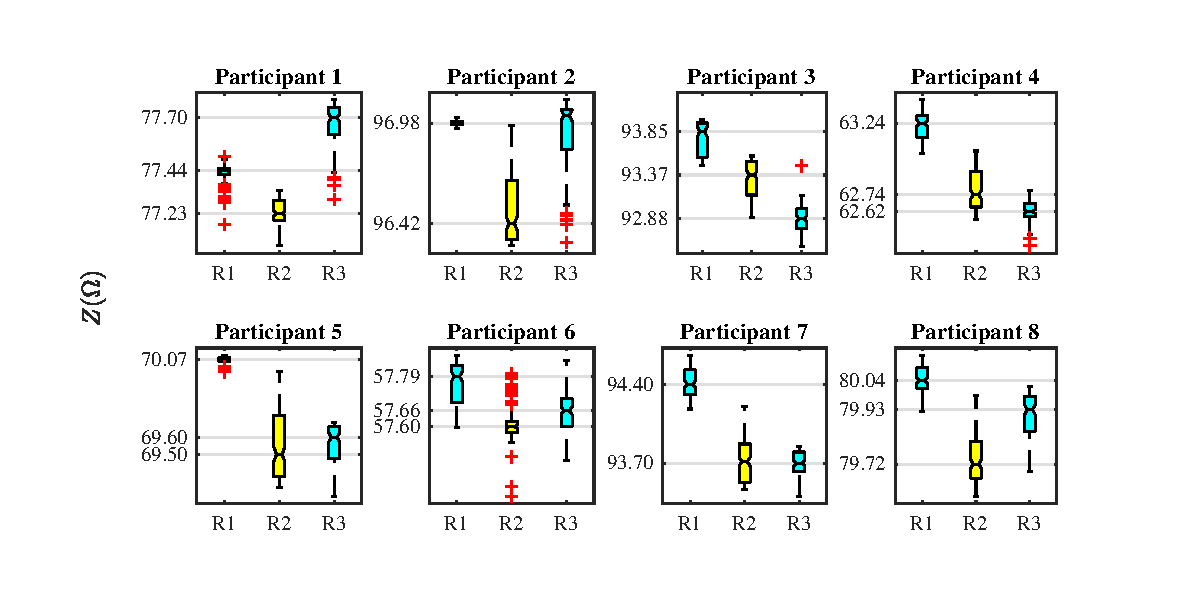
\includegraphics[width=15cm,keepaspectratio]{figure_vop_1}    
	\caption[Change of impedance during venous occlusion]{Box plot showing the statistical change of impedance in $\Omega$ during venous occlusion. The cyan boxplot represents the baseline before (Region 1) and after (Region 3) the occlusion. The yellow marker is the impedance during venous occlusion (Region 2).}
	\label{fig:venous statistics impedance}
\end{figure}  

Figure \ref{fig:venous occlusion impedance} shows the deviation of the impedance in terms of change in percentage of impedance ($\Delta Z\%$) from the median baseline in region 1. The shaded area represents the venous occlusion between \SIrange{300}{400}{\second}. The dots are the points of the foot of the signal equivalent to ($R_B$). The signal was smoothed using the command \textit{smooth} in Matlab which assigns a lower weight to outliers in the regression. This method assigns zero weight to data outside six mean absolute deviations \cite{MATLAB:2016}. Hence, it eliminates most of the rapid variations of impedance caused by motion artefact. 

\begin{figure}[htbp]
	\centering
	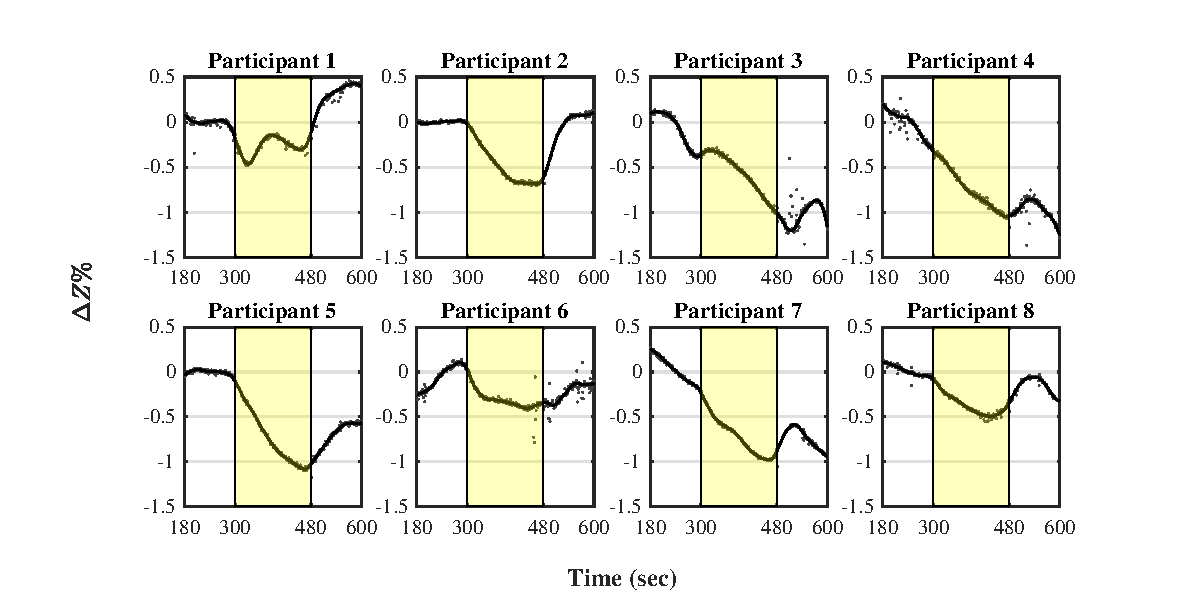
\includegraphics[width=15cm,keepaspectratio]{figure_vop_2}    
	\caption[Percentile variation of impedance during venous occlusion]{Percentile change of impedance during venous occlusion. The reference baseline is the average baseline impedance during the last \SI{2}{\minute} before the venous occlusion.}
	\label{fig:venous occlusion impedance}
\end{figure} 

The figure clearly reveals a linear trend during venous occlusion for most of the subjects. Nonetheless, participant's 1 resistance fell immediately as the occlusion occurred but a minute later, the participant moved his arm reversing the trend. Later on, the impedance continued decreasing again. Furthermore,  participant 6 also showed a similar response when the individual moved his arm, but in his case, the resistance settled instead of reversing the trend. Interestingly, participant 2 showed a saturation point after quite a few seconds, which it was particular of this subject. 

The table \ref{tbl:vop delta impedance} summarises the changes of impedance during the venous occlusion. The average median of the resistance drop from the baseline value was roughly \SI{-0.546(0076)}{\%}, where participants 4, 5 and 7 recorded the largest loss of impedance (>\SI{0.5}{\%}). The column \textit{Change} on the same table shows the impedance difference from the initial occlusion point to the minimum point of the smooth curve, calculated using equation \ref{eq:DeltaZ}. It revealed that during the venous occlusion the whole slope recorded a variation of \SI{0.658(0230)}{\percent}.

\begin{align}
	\label{eq:DeltaZ}
	\Delta Z\%_T = \Delta Z\%_{300 sec} - \Delta Z\%_{min}
\end{align}


\begin{table}[htbp]
	\caption[Statistical analysis of the percentile change of impedance during venous occlusion]{Statistical analysis of the percentile change of impedance during venous occlusion. The data represents the median percentile change of impedance per participant, the maximum and minimum value of the occlusion and the difference between these two peak values.}
	\label{tbl:vop delta impedance}
	\centering
	\begin{tabular}{l@{\hspace{1cm}}
			S[table-format=-1.2]@{\,\( \pm \)\,}
			S[table-format=1.2]
			c
			c
			c}
		\toprule
		&\multicolumn{2}{c}{\textbf{Median}}  
		&\textbf{Max} 
		&\textbf{Min}
		&\textbf{Change} \\ 
		&\multicolumn{2}{c}{\textbf{[$\Delta Z \%$]}}
		&\textbf{[$\Delta Z \%$]}
		&\textbf{[$\Delta Z \%$]}
		&\textbf{[$\Delta Z \%$]}\\\midrule
		Participant 1 & -0.26 & 0.09 & -0.20 & -0.47 & 0.26 \\ 
		Participant 2 & -0.58 & 0.21 & -0.03 & -0.69 & 0.66 \\  
		Participant 3 & -0.51 & 0.22 & -0.35 & -1.00 & 0.66 \\  
		Participant 4 & -0.79 & 0.22 & -0.32 & -1.06 & 0.74 \\ 
		Participant 5 & -0.82 & 0.30 & -0.11 & -1.09 & 0.98 \\  
		Participant 6 & -0.33 & 0.09 &  0.03 & -0.41 & 0.43 \\  
		Participant 7 & -0.72 & 0.22 & -0.22 & -0.98 & 0.77 \\  
		Participant 8 & -0.40 & 0.11 & -0.09 & -0.50 & 0.41 \\  
		\bottomrule
	\end{tabular} 
\end{table}		  

It is alluring to note the immediate change of impedance as soon as the venous occlusion occurs. The capability of impedance plethysmography device to detect venous  occlusion in all the participants is remarkable and almost instantaneous. As soon as the blockage occurs the impedance drops for some time, if motion does not change the trend, some could reached saturation as seen on participant 2. However, it is also apparent that other signals also reached a point of saturation, portraying a decrease of impedance in an exponential trend than linear. 

This effect can be summarised in figure \ref{fig:venous occlusion change}. This plot describes the change of impedance in time ($dZ/dt$) against some data points (beats) during the venous occlusion. For this, 10 data points of $R_B$, which are synchronised with the heart cycle, were clustered computing $dZ/dt$. This differential value is equivalent to the velocity of change of the basal impedance per second (\si{\ohm\per\second}). In general the average impedance all along the whole occlusion was \SI{-0.0026(00018)}{\beats}.

\begin{figure}[htbp]
	\centering
	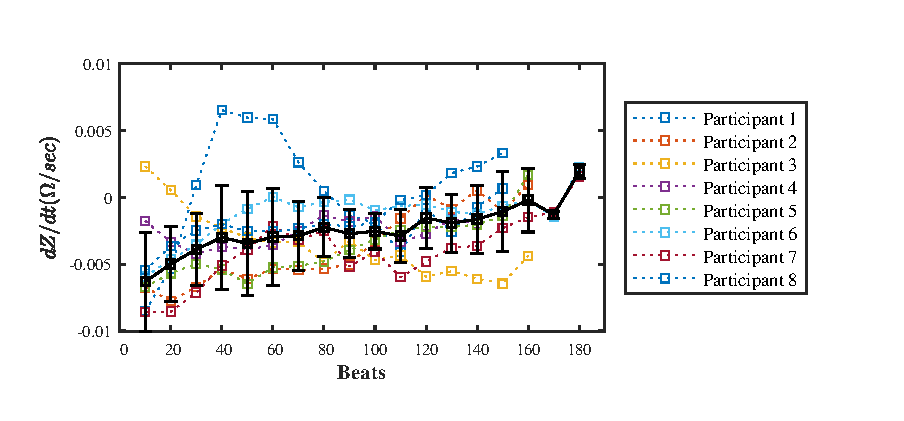
\includegraphics[width=15cm,keepaspectratio]{figure_vop_3}    
	\caption[Rate of change of impedance per 10 heartbeats during venous occlusion]{Speed of change of impedance in time ($dZ/dt$) per every 10 heartbeats. The colour lines represent the data per each participant. The dark bold line is the mean of all the measurements.}
	\label{fig:venous occlusion change}
\end{figure}

From the figure can be concluded that during the first 10 beats, there is a higher drop of impedance compared to the last data points. Indeed, the rate of change of resistance in the first 10 beats was in average \SI{-0.0063(00037)}{\Omega\per\second}. After 90 beats the result of the derivation was more than halved to an average of \SI{-0.0027(00018)}{\Omega\per\second}. At 160 beats the ratio was reduced to just \SI{-0.0002(00024)}{\Omega\per\second}. The final data points (180 beats) showed a reversion of the trend (\SI{0.0019(0005)}{\Omega\per\second}). However, this is due to the just few participants achieved that amount of heart beats.  Moreover, at this point some data were already returning to baseline because the cuff could have been released few seconds earlier.  


%%********************************** % Section 7.1.2 ******************************************
\subsection{Change of impedance during partial arterial occlusion}
\label{section occlusion 1.2}
The same analysis performed on the VOP was applied to the partial arterial occlusion. The partial restriction of the arterial blood flow is achieved by mechanically occluding the upper arm between diastolic and systolic pressures. The load levels used to create these occlusions are detailed on the column \textit{occlusion 2} in the table \ref{tbl: venous occlusions}. Similar time lapses were used to analyse the data, the last \SI{2}{\minute} of the region 3 (\SIrange{660}{780}{\second}), the whole partial arterial blockage in region 4, \SI{3}{\minute} between \SIrange{780}{960}{\second}, followed by \SI{2}{\minute} of return to baseline after releasing the pressure of the cuff in region 5 (\SIrange{960}{1080}{\second}).

Occluding the blood flow at this pressure level induced an uncomfortable feeling on the participants, some of them felt numbness in their arms during the study. Therefore, some partakers moved their arms like participant 1, in others, the length of the occlusion had to be shortened like in participant 4 where the occlusion occurred later (\SIrange{840}{960}{\second}) because ECG sensors had to be relocated and participant 8 who asked to terminate the blockage a minute earlier (\SIrange{780}{900}{\second}). 

During this kind of occlusion, there is no venous return, as well as the inflow being slightly restricted. Indeed, the occlusion constricts the brachial artery where only a  small amount of blood passes through the obstruction. Moreover, the blood flow becomes turbulent after the cuff's constriction.  Due to the venous occlusion action, it is expected the arm to increase its volume as blood pools in the forearm reducing the basal impedance. 

Figure \ref{fig:partial arterial statistics impedance} confirms the reduction of the basal impedance all along partial arterial occlusion. Comparable to VOP, the box-plot shows a larger upper and lower quartile distribution for most of the participants in region 4, because of a continued drop in basal impedance during that occlusive action. However, partaker 4 depicted a significant number of outliers, which was mainly caused by motion artefact. The data also reports that only a few participants were able to get back close to baseline resistance, such as participants 2 and 7. Interestingly, some study members displayed a swift recovery in the region 5. For instance, the large data distribution in participants 1, 2, 4, 6, 7 and 8 describes a fast trend to return to baseline. But in general terms, it seems that a longer recovery time is required to return to an impedance value close to baseline after partial arterial occlusion. 

\begin{figure}[htbp]
	\centering
	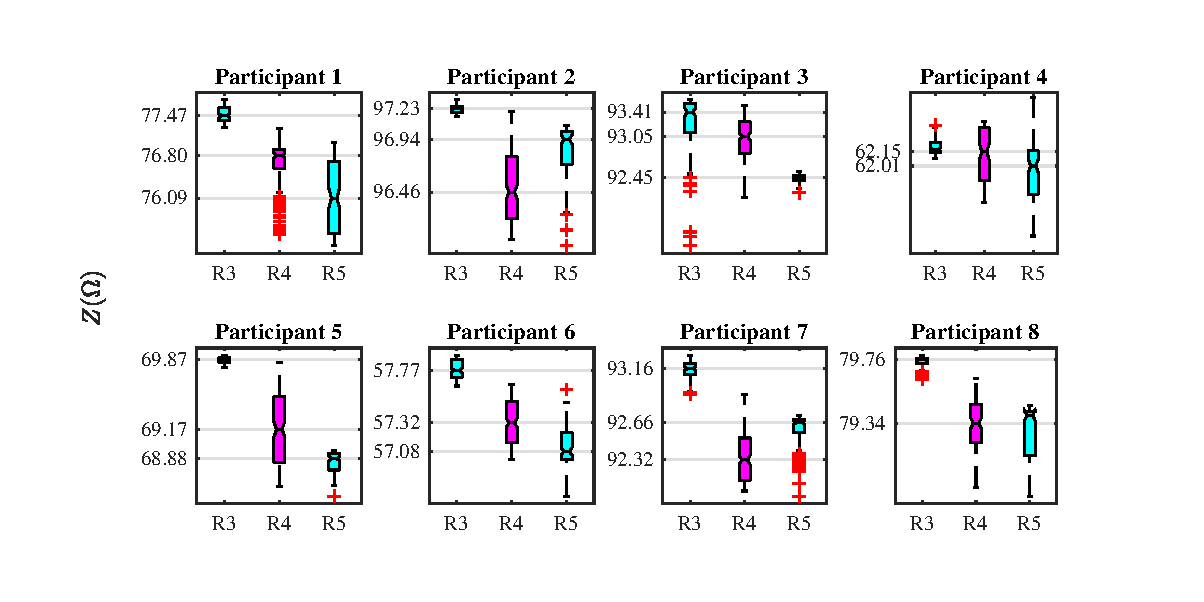
\includegraphics[width=15cm,keepaspectratio]{figure_vop_4}    
	\caption[Change of impedance during partial arterial occlusion]{Boxplot of the statistical change of impedance in $\Omega$ during partial arterial occlusion. The cyan marker represents the baseline before (Region 3) and after (Region 5) the occlusion. The magenta marker is the impedance during partial arterial occlusion (Region 4).}
	\label{fig:partial arterial statistics impedance}
\end{figure}  

By qualitatively analysing the change of impedance by percentage from baseline region 3, figure \ref{fig:arterial occlusion imepdance} displays that there is a linear trend during the cuff's pressure in the region 4. Certainly, it can be noticed that the impedance drop is more pronounced than the one from venous occlusion (see figure \ref{fig:venous occlusion impedance}). In participant 1 the motion artefact is more evident, the step drop of basal impedance right before the release of the cuff's pressure is a reflection of the muscular movement of his forearm. In this case, it is evident that the arm movement augmented the change of impedance throughout the occlusion. However, other participants also experienced motion artefact, but the change of impedance was just within a few heart beats. For instance, participant 2 showed only a data point off the smooth line, but in participants 3 and 4, the amount of data points off the soft signal were significantly larger. But in summary, most of the participants described a straight drop of impedance, especially linear in participants 2 and 5. 

After releasing the cuff's pressure, it is easy to see that most of the signals change the slope of the signal. The only one that did not reflect this change was participant 3. This impedance correction reflects the restoration of the blood circulation and the reduction of the forearm's volume. Moreover, there is not an apparent settling impedance value, except for participant 7 and 8. In general, this change of trend also confirms that the body might require longer to recover after the partial arterial occlusion.

\begin{figure}[htbp]
	\centering
	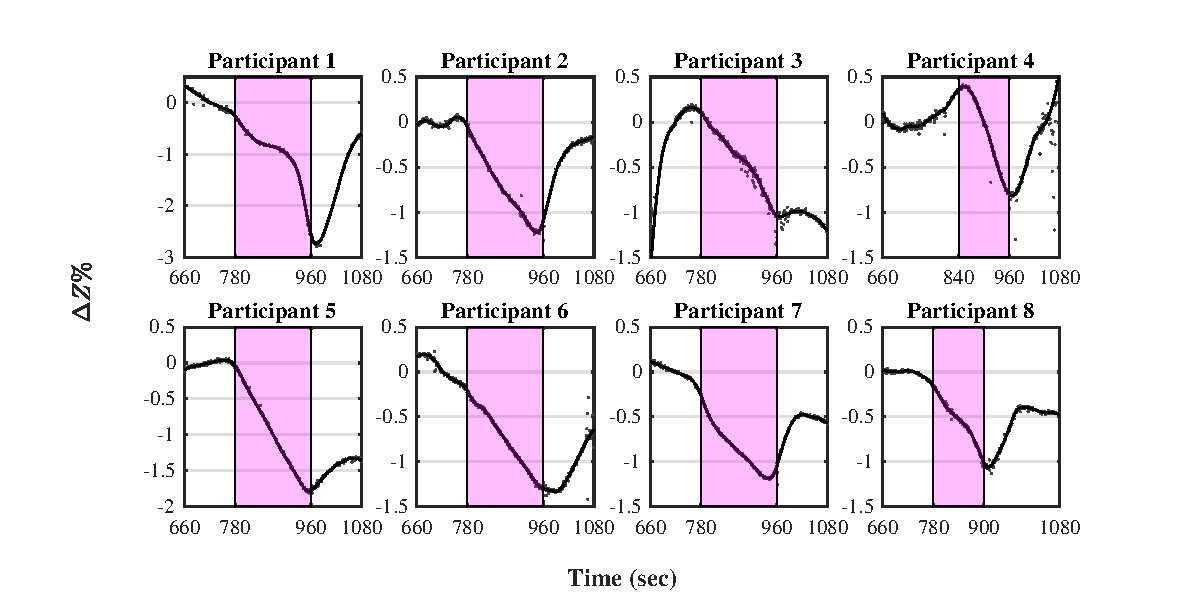
\includegraphics[width=15cm,keepaspectratio]{figure_vop_5}    
	\caption[Percentile variation of impedance during partial arterial occlusion]{Percentile change of impedance during partial arterial occlusion, using as reference average baseline impedance during the last \SI{2}{\minute} before the occlusion.}
	\label{fig:arterial occlusion imepdance}
\end{figure}  

Table \ref{tbl:AO delta impedance} reports the percentage variations from the baseline impedance in region 3 in more depth. The median impedance drop from the baseline was approximately \SI{-0.783(0324)}{\percent}. However, participant 4 showed a lower median value, because of the initial impedance value was above the baseline average at \SI{0.34}{\percent}. Evidently, there is a larger reduction of impedance or increase of the forearm's volume rather than VOP. The median change of impedance from the maximum to the minimum value was around \SI{1.133(0482)}{\percent} which is nearly double when compared to venous occlusion. A  physiological response might have caused this increase in volume. The blood pooling could not cause this increase of volume because the arterial blood flow was restricted, so less amount blood entered into the forearm segment. 

\begin{table}[htbp]
	\caption[Statistical analysis of the percentile change of impedance during partial arterial occlusion]{Statistical analysis of the percentile change of impedance during partial arterial occlusion. The data represents the median percentile change of impedance per participant, the maximum and minimum value during the occlusion and the difference between these two peak values.}
	\label{tbl:AO delta impedance}
	\centering
	\begin{tabu}{l@{\hspace{1cm}}
			S[table-format=-1.2]@{\,\( \pm \)\,}
			S[table-format=1.2]
			c
			c
			c}
		\toprule
		&\multicolumn{2}{c}{\textbf{Median}}  
		&\textbf{Max} 
		&\textbf{Min}
		&\textbf{Change} \\ 
		&\multicolumn{2}{c}{\textbf{[$\Delta Z \%$]}}
		&\textbf{[$\Delta Z \%$]}
		&\textbf{[$\Delta Z \%$]}
		&\textbf{[$\Delta Z \%$]}\\\midrule
		Participant 1 & -0.85 & 0.50 & -0.28 & -2.56 & 2.29 \\  
		Participant 2 & -0.80 & 0.35 & -0.05 & -1.23 & 1.18 \\  
		Participant 3 & -0.38 & 0.32 &  0.10 & -1.04 & 1.14 \\  
		Participant 4 & -0.03 & 0.41 &  0.34 & -0.78 & 1.13 \\  
		Participant 5 & -1.01 & 0.54 & -0.04 & -1.80 & 1.76 \\  
		Participant 6 & -0.77 & 0.33 & -0.21 & -1.30 & 1.09 \\  
		Participant 7 & -0.90 & 0.26 & -0.25 & -1.19 & 0.93 \\  
		Participant 8 & -0.53 & 0.22 & -0.15 & -1.01 & 0.85 \\  
		\bottomrule
	\end{tabu} 
\end{table}	

\begin{figure}[!t]
	\centering
	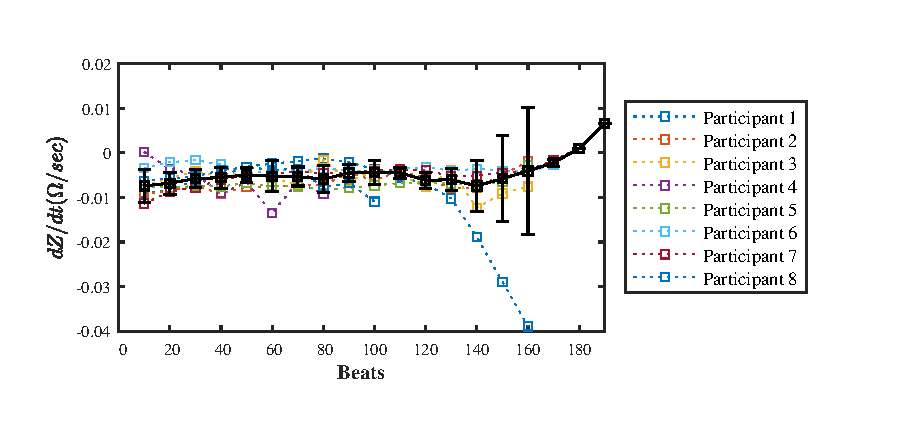
\includegraphics[width=15cm,keepaspectratio]{figure_vop_6}    
	\caption[Rate of change of impedance per 10 heartbeats during partial arterial occlusion]{Speed of change of impedance in time per every 10 heartbeats. The colour lines represent the data per each participant. The dark bold line is the mean of all the measurements.}
	\label{fig:arterial occlusion change}
\end{figure}  

The calculation of the velocity of the change of impedance  ($dZ/dt$) displayed a similar exponential response as in VOP. Figure \ref{fig:arterial occlusion change} shows the calculation of these points for all the participants. The plot indicates that the first 10 beats of changed on a ratio average of \SI{-0.0074(00037)}{\Omega\per\second} which was the largest acceleration. Then between 20 and 110 beats the velocity stabilised to \SI{-0.0053(00007)}{\Omega\per\second}. After this apparent settling, there is a new increase in the differentiation. However, it seems to be aided by the motion artefact seen on participant 1 for a few beats.

%%********************************** % Section 7.1.3 ******************************************
\subsection{Impedance variation during total occlusion}
\label{section occlusion 1.3}
The blood supply towards the forearm was completely blocked by inflating the cuff above systolic pressure, in the case of this study \SI{20}{\mmHg} above this point. The column \textit{occlusion 3} in the table \ref{tbl: venous occlusions} shows the pressure level applied for the research. The data regions involved in this part of the investigation were regions 5, 6 and 7. Equally to previous occlusions analysis, the last 2 minutes of data from region 5 were used as impedance baseline (between \SIrange{1140}{1260}{\second}). Then, the cuff was inflated to accomplish complete blood flow obstruction; the occlusion was maintained for \SI{3}{\minute} between \SIrange{1260}{1440}{\second}. Finally, the cuff's air was immediately released, and readings were taken for further \SI{2}{\minute}.

This test caused a lot of discomfort to most of the participants, numbness and willingness to move their limb was common for all the participants. Hence, they ended up moving their arms voluntarily. Because there is no either blood flowing or pooling during this part of the experiment, it was expected small impedance variations. Additionally, the mean restive value would be equivalent to the impedance of the tissue's components within the segment plus the impedance of the residual blood in the forearm. However, when a change of resistivity happens, this is mostly caused by the participant's re-accommodation rather than a physiological variable. 

Figure \ref{fig:total arterial statistics impedance} shows how the impedance change during the total occlusion. Initially, it can be seen that there was not a consensus on the signal trend all along the occlusion as seen on the previous tests.  Some of the participants reflected a small reduction in their median impedance, like study members 1,  4, 5, 6 and 8, whereas the rest experienced a slight increase of it. Also, the trend of the signal during the occlusion is not clear; different signals have different data distribution points, for instance,  participant 1 and 7 displayed a large data distribution indicating a constant change of their median impedance. On the other hand, the rest showed a data distribution centred in the median, illustrating a little impedance variation during the occlusion. Only participant 5 exhibited a significant number of outliers, representing rapid changes at one point of the measurement. In general, there is not a linear trend as reported by the other kind of occlusions. 

\begin{figure}[!hpb]
	\centering
	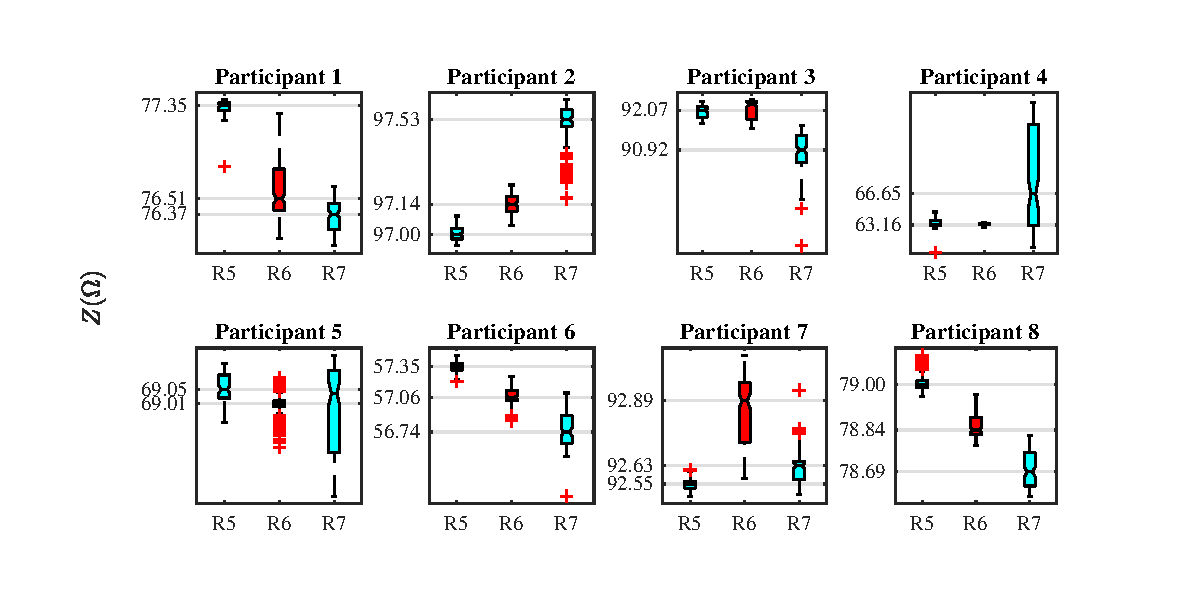
\includegraphics[width=15cm,keepaspectratio]{figure_vop_7}    
	\caption[Change of impedance during total occlusion]{Boxplot of statistical change of impedance in $\Omega$ during total occlusion. The cyan marker represents the baseline before (Region 5) and after (Region 7) the occlusion. The red marker is the impedance during total occlusion (Region 6).}
	\label{fig:total arterial statistics impedance}
\end{figure} 

After releasing the cuff's pressure, again there is not a definite trend in the direction of the impedance. Some of the participants displayed an increase of their resistivity. However, participants 4 and 5 presented exaggerated impedance changes. It is not clear the nature of this rare variation, but it could be due to the limb movement after the occlusion. Moreover, there is not a quick change of impedance as experienced on the other type of occlusions. Which, somehow is congruent with the fact that there is no blood rushing in or out of the forearm.

By analysing the variation of impedance during the occlusion compared to the baseline (region 5), it can be seen the magnitude and direction of the resistivity change. Evidently, participant 1 displayed the largest and continuous impedance decrease which is unusual for this type of occlusion. Another unexpected resistivity response was the one performed by participant 7 where his impedance increased in a small proportion.  

The table \ref{tbl:TO delta impedance} describes in detail the impedance changes during the occlusion. The median impedance during total occlusion was \SI{-0.135(0441)}{\percent} which is quite close to zero. However, the sign of column \textit{median} indicates that five out of eight exhibited a negative trend in the impedance direction, indicating resistivity loss. In fact, most of the measurements were below \SI{0.5}{\percent}, only participants 1 and 5 showed the higher changes of impedance. By calculating the $\Delta \%$  from the maximum and minimum changes (column \textit{Change}) can be deducted that only participant 1 presented a change greater than \SI{1}{\percent}, between \SIrange{0.5}{1}{\percent} participant 3 and 6 displayed this data range and the rest were below \SI{0.5}{\percent}. In general, the changes described by total occlusion were significantly lower than the other occlusions indicating a minimum increase of volume, for instance partakers 2 and 5 median impedance were a clear illustration of this. Some changes of impedance were presented in some measurements which can be related to a muscular activity. 

\begin{figure}[htbp]
	\centering
	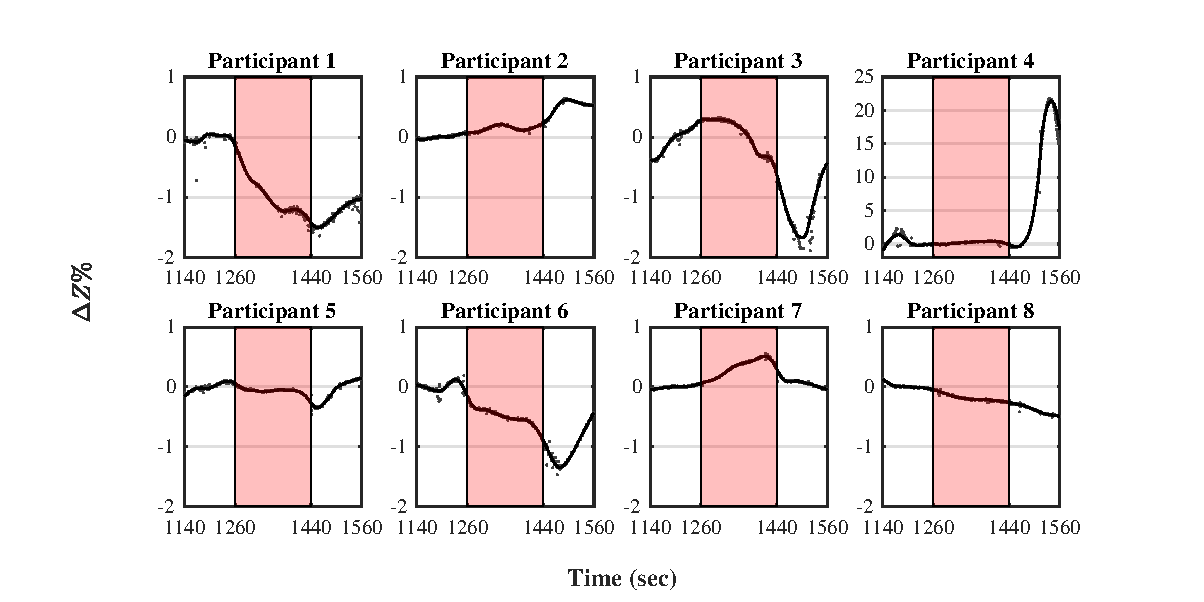
\includegraphics[width=15cm,keepaspectratio]{figure_vop_8}    
	\caption [Percentile variation of impedance during total occlusion]{Percentile change of impedance, using as reference average baseline impedance during the last \SI{2}{\minute} before the total occlusion.}
	\label{fig:total occlusion imepdance}
\end{figure} 

\begin{table}[htbp]
	\caption[Statistical analysis of the percentile change of impedance during total occlusion]{Statistical analysis of the percentile change of impedance during total occlusion. The data represents the median percentile change of impedance per participant, the maximum and minimum value during the occlusion and the difference between these two peak values.}
	\label{tbl:TO delta impedance}
	\centering
	\begin{tabu}{l@{\hspace{1cm}}
			S[table-format=-1.2]@{\,\( \pm \)\,}
			S[table-format=1.2]
			c
			c
			c}
		\toprule
		&\multicolumn{2}{c}{\textbf{Median}}  
		&\textbf{Max} 
		&\textbf{Min}
		&\textbf{Change} \\ 
		&\multicolumn{2}{c}{\textbf{[$\Delta Z \%$]}}
		&\textbf{[$\Delta Z \%$]}
		&\textbf{[$\Delta Z \%$]}
		&\textbf{[$\Delta Z \%$]}\\\midrule
		Participant 1 & -1.09 & 0.33 & -0.14 & -1.38 & 1.24 \\  
		Participant 2 &  0.14 & 0.04 &  0.07 &  0.07 & 0.00 \\  
		Participant 3 &  0.18 & 0.28 &  0.30 & -0.50 & 0.81 \\  
		Participant 4 &  0.21 & 0.16 &  0.05 & -0.14 & 0.19 \\  
		Participant 5 & -0.06 & 0.05 &  0.05 & -0.23 & 0.28 \\  
		Participant 6 & -0.51 & 0.14 & -0.15 & -0.89 & 0.75 \\  
		Participant 7 & -0.36 & 0.15 &  0.05 &  0.05 & 0.00 \\  
		Participant 8 & -0.21 & 0.06 & -0.05 & -0.27 & 0.22 \\  
		\bottomrule
	\end{tabu} 
\end{table}	

Figure \ref{fig:total occlusion change} illustrates the analysis of the velocity rate ($dZ/dt$) which the basal impedance changes. It clearly reflects that participant 1 basal impedance decreased swiftly compared to the rest of the partakers. Also, participant 3 experienced a quick impedance drop between \SIrange{80}{140}{\beats}. In general, the average velocity for the total occlusion was around \SI{-0.00061(000170)}{\Omega\per\second} which is considerably small compared to the other occlusions. However, at the beginning of the occlusion, there was a modest increase in the velocity, the average for the first \SI{10}{\beats} was around \SI{-0.0027(00052)}{\Omega\per\second}. After that, it stabilised close to the median value of all the measurements until \SI{140}{\beats}. Nonetheless, between \SIrange{140}{180}{\beats} there was an increase in the velocity due to the contribution of the negative trends before releasing the occlusion. 

\begin{figure}[htbp]
	\centering
	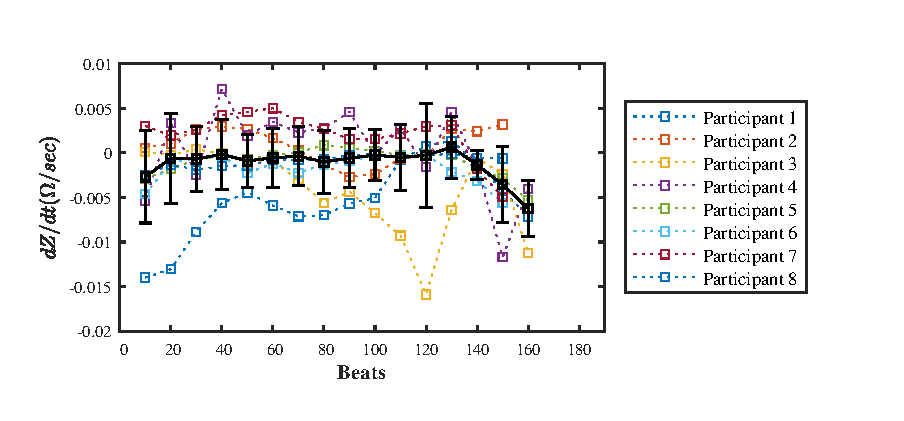
\includegraphics[width=15cm,keepaspectratio]{figure_vop_9}    
	\caption[Rate of change of impedance per 10 heartbeats during total occlusion]{Speed of change of impedance in time per every 10 heartbeats during total occlusion. The colour lines represent the data per each participant. The dark bold line is the mean of all the measurements.}
	\label{fig:total occlusion change}
\end{figure} 

%%********************************** % Section 6.5 ******************************************
\section{Conclusion}
\label{senction basal conclusion} 

There are different tissues in the body contributing to the impedimetric signal like fat, muscle, blood and bone. Most of these organs or tissues have intrinsic impedances. The sum of all these resistive values is known as basal impedance. The data collected showed that the geometry of the forearm segment altered the impedance reading, showing an inverse relation between the volume of the segment and the average impedance. The device designed took measurements within the expected ranges of a human forearm. However, motion artefact or the interface electrode-skin may contributed to shifting the resistance value of the measurement. The basal impedance varied from the median measurement in average \SI{-0.6384}{\percent} with a maximum deviation of \SI{-2.353}{\percent}. After performing a statistical analysis of these variances, it was found that any values within $\pm 1.66 \%$ are within statistical normal values. 

From the point of view of detection of circulatory problems, the experimental task showed that it is evident that the basal impedance changed linearly when an occlusion in the forearm occurred. By occluding the venous return and not altering the arterial flow, blood can enter into the limb but cannot leave. As a result, the volume of the forearm increased constantly while the occlusion took place. Hence, this gain of capacity can be quantified by the impedimetric method as a variation of the basal impedance median value. As blood cell population increased, the conductivity of the forearm section also rose in value. Therefore, the resistivity proportionally decreased.

During the occlusive events the iPG device detected changes of impedance magnitude due to the pooling effect caused by the constriction of the upper arm. Clearly, the basal impedance decreased during venous and partial occlusion. Interestingly the impedance changed at different ratio when venous and partial arterial occlusion were applied. The impedance during VOP varied in a \SI{0.658(0230)}{\percent}. On the other hand, all along PAO the impedance changed in \SI{1.13(0482)}{\percent}. This greater slope might indicate a higher increase of blood volume but this might be incorrect because restricting the brachial artery reduces the flow towards the distal section of the arm \cite{mccully2004muscle}. This data points out that an arterial occlusion might be represented in a fast drop of impedance, whereas in a venous occlusion the impedance might drop at slower pace. In contrast, during total occlusion the impedance did not change as dramatically compared to the other episodes. The impedance went in different directions with no common trend identified. This effect might have been caused by forearm accommodation rather than a physiological response. In average the ratio change was well below the other occlusions around \SI{0.250(0446)}{\percent}. 

Analysing the acceleration of the blood during the occlusions, it was found that after the upper arm occlusion during the first 10 heartbeats the impedance changed faster than the rest of the test. During these heartbeats, the change of impedance was around \SI{-0.0063(00037)}{\Omega \per \second} for venous occlusion, quite closely partial arterial occlusion was about \SI{-0.0074(00037)}{\Omega \per \second}, and total occlusion was \SI{-0.0027(00052)}{\Omega \per \second}. This acceleration might indicate a physiological response of the veins to allow extra blood in the forearm. Some studies \cite{joyner2001belfast, hainsworth2003syncope} suggest that the increase of blood flow may be related to a syncopal response. As a a regulatory response of the human body. Nonetheless, further research must be performed to corroborate these assumptions. 

All along total occlusion (Region 6) seemed that there was not a clear decline or increase of basal impedance common to all the participants. In general the change of impedance was around \SI{-0.135(0441)}{\percent}. A reason for this value close to zero was that neither arterial nor venous blood was flowing through the limb, thus not change of volume was produced. In the end, this value was the real basal impedance where all the tissues with their blood content were measured. The information obtained here is an indicator of development of ischemia. A study have demonstrated that when total occlusion occurs cells starvation take place ischemia develops \cite{ristic1997muscle} which could be detected as a decrease in the basal impedance. 


%********************************** %Nomenclature found  *************************************
\nomenclature[z-pdf]{PDF}{Probability density function}
\nomenclature[z-PAO]{PAO}{Partial arterial occlusion}